\section{Introduction to Organization}
Auribises offers a suite of mobile, web and software applications as a solution to industry.
\begin{figure}[ht]
\centering
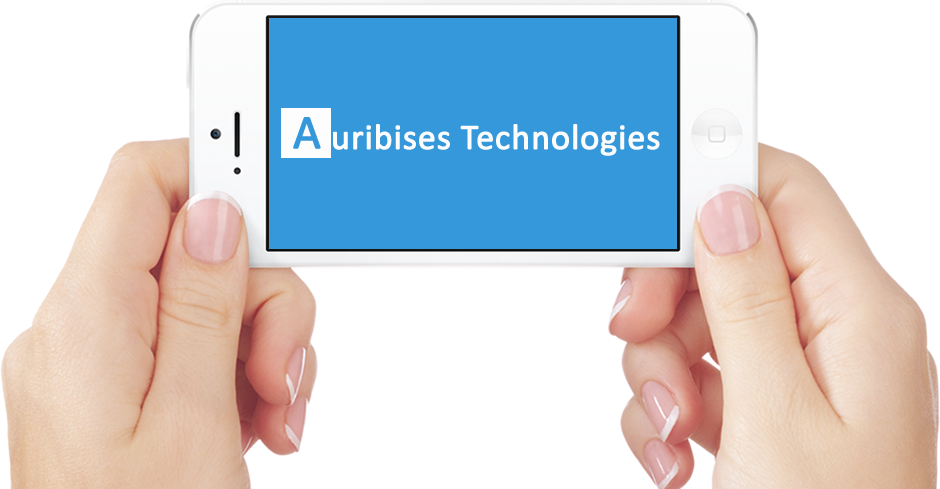
\includegraphics[scale=0.3]{images/aur.png}
\caption{Auribises}
\end{figure} 
We were founded in November 2011. With unparalleled domain competencies in mobile and web, Auribises is poised to take on critical challenges that the industry manifests. Our culture is values based, and we assure the highest ethical standards of integrity, transparency and corporate governance. Our value system is driven by STAR, the acronym for our core values of Share, Time, Achieve, and Respect. At Auribises, we just not only develop, but also provide educational services that helps students to hone their technical skills. Auribises offers a unique combination of technical competencies with practical exposure on ongoing projects to its students. Auribises has a core vision for lightening thousands of candles with a single candle and hence we believe that it is our endeavor to continually share our learning’s with the larger world.
\section{Introduction To Project} 
With the launch and increase in sales of smartphones over the last few years, people are using
mobile applications to get their work done, which makes their lives easier. Mobile applica-
tions comprise various different categories such as Entertainment, Sports, Lifestyle, Education,
Games,Food and Drink, Health and Fitness, Finance, etc. The application falls under Sports
category and helps the students to access all the news related to sports department of Guru
Nanak Dev Engineering College , Ludhiana .
The applications interface is designed using custom art elements, the functionality is imple-
mented using Android SDK, and the phase of testing the product was accomplished success-
fully. The application can very well manage,store and share different news related to sports
among different users.Students who are Sports enthusiastic can get full information of sports
department.Admin panel can upload news and student panel can view those news in the mo-
bile. Description of sports depatment such as commitee menbers , facilities , scholarships ,
achievements and other optional attributes ( Adding latest news to the in applications). All
these topics have been explained in detail in their respective chapters.

\section{Project Category(Internet based, Application or System Development)}
This application is android mobile application based on internet using real time NoSql database(Firebase Database).

\section{Objectives}

\begin{itemize}
	\item  To design application that can full fledged information about sports department.

	\item Acknowledging students who got various achievement in the sports..
	
	\item Sports enthusiast can get news uploaded by the sports department easily.


\end{itemize}

\section{Problem Formulation}
An easy and stable platform for students who loves to take part in different sports activities. Helpful for the students, for accessing latest news uploaded by the department. They can easily contact the department commitee anytime and can register to participate in the games. 

\section{Proposed System Modules}

\begin{itemize}
	\item Latest news of sports department can be Upload ,Share , Delete.

	\item Acknowledgement of students under various sports category.
	
	\item Login Page(To ensure authenticated and secure system, system will have a login activity to ensure that only authorized user can use this system).
	
	\item Find location through map option.
	


\end{itemize}

 
\section{Unique Features of the System}
\begin{itemize}

\item Adding latest news in various categories.
\item Acknowledging students who got various achievement in the sports.
\item Admin can delete the news uploaded by him/her.
\item Students can register through our application to participate in different games .
\item Students gets all the information regarding sports facilities available in the college.
\item User can share the App with anyone.
\end{itemize}


